\section{Gain Layer Experiments}\label{sec:ch6:gainlayer_experiments}
Before we explore the possibilities and performance of using a
nonlinearity in the wavelet domain, let us present some experiments and results
for the wavelet gain layer where we do nonlinearities purely in the
spatial domain, as in a conventional CNN layer. This is the first objective in
\autoref{sec:ch6:learning}, comparing $G$ to $H$.

\subsection{CNN activation regression}\label{sec:ch6:regression}
\begin{figure}[t]
  \centering
  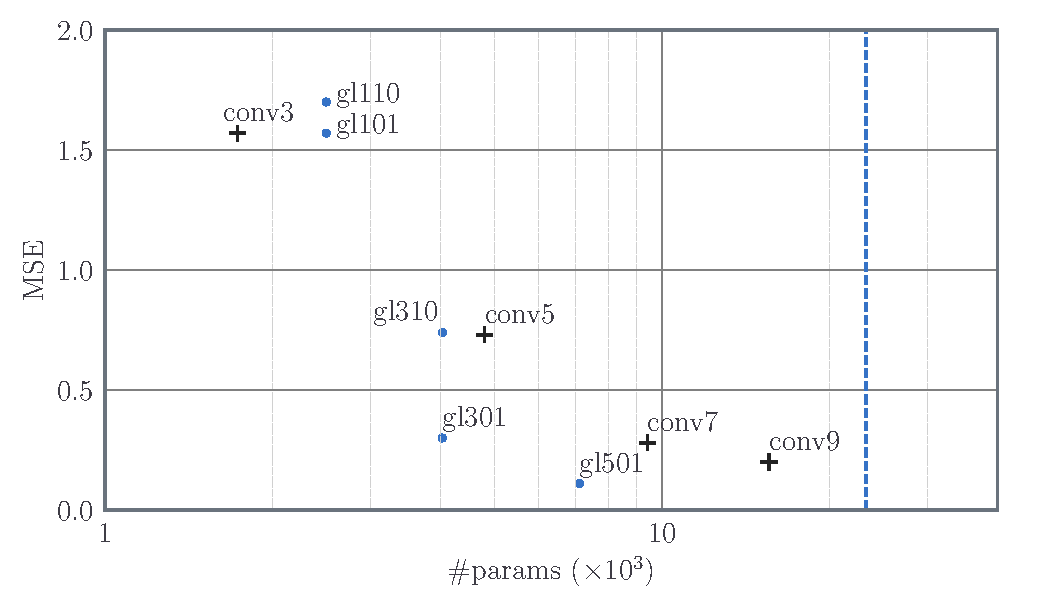
\includegraphics[width=\textwidth]{\imgpath/AlexNet_layer1_regression.pdf}
  \mycaption{Normalized mean squared error for conv layer and wavelet gain layer
  regression}{We minimize
  \eqref{eq:ch6:conv_regression} and
  \eqref{eq:ch6:gain_regression} on the ImageNet validation set, where the
  target is made from convolving the input with AlexNet's first layer filters.
  This plot shows the final NMSE score compared
  to the number of learnable parameters. The original conv layer has spatial
  support $11\x 11$. The four points labelled `conv$n$' correspond to filters with
  $n\x n$ spatial support. The four points labelled `gl$abc$' correspond to two-scale
  gain layers with $a\x a$ support in the lowpass, $b\x b$ spatial support
  in the first scale, and $c\x c$ spatial support in the second scale. The gain
  layer can regress to the AlexNet filters quite capably. In this example, it is
  important to have at least $3\x3$ lowpass support for the gain layer, and the
  second scale coefficients are more important than the first scale.}
  \label{fig:ch6:gainlayer_regression}
\end{figure}
One of the early inspirations for using wavelets in CNNs was the visualizations
of the first layer filters learned in AlexNet. These $11\x 11$ colour filters
(see \autoref{fig:ch1:alex_filt}) look very much like a 2-D oriented wavelet transform.

So how well can the gain layer emulate the action of this layer? How would it
compare to trying to use a reduced size convolutional kernel to learn the
action of the layer?

Let us call the action of our target layer $H_0$, a learned convolutional layer $H$
and our gain layer $G$.
% Let $\lnorm{H}{2}$, $\lnorm{G}{2}$ be the $\ell_2$ norm
% of the weights for each layer.
We assume that we do not have direct
access to $H_0$ but only the convolved outputs $Y=H_0 X$. Then, we would like to solve:
\begin{align}
  & \argmin_{H}\ (Y - HX)^2 %+ \frac{\lambda}{2} \lnorm{H}{2}^2
  \condition{s.t. $h[c, \nn] = 0,\ \forall \nn \notin \mathcal{R}$} \label{eq:ch6:conv_regression}\\
  & \argmin_{G}\ (Y - \mathcal{W}^{-1}G\mathcal{W}X)^2 %+ \frac{\lambda}{2} \lnorm{G}{2}^2
  \condition{s.t. $g_{j,k}[c, \nn] = 0,\ \forall \nn \notin \mathcal{R'}$} \label{eq:ch6:gain_regression}
\end{align}
for some support regions $\mathcal{R},\mathcal{R'}$. E.g. $\mathcal{R}$ is a $3\x3$ or $5\x5$
block, and similarly $\mathcal{R'}$ is a $1\x 1$ region in each
subband.

\eqref{eq:ch6:conv_regression} and \eqref{eq:ch6:gain_regression} are both
regression problems convex in the parameters of $H$ and $G$, with many possible
ways to solve. We are not worried with the optimization procedure chosen here,
but of the final distances $\norm{Y-HX}$ and $\norm{Y-\mathcal{W}^{-1}G\mathcal{W}x}$ (or
equivalently, their squares). We choose to find $H$ and $G$ by gradient descent,
using the validation set for ImageNet as the data input-output pair $(X, Y)$.
After 3--5 epochs, both $H$ and $G$ typically settle into their global minimum.
Because of the large size of the input filters, we allow for both a $J=1$ and
$J=2$ scale gain layer but only learn weights at the lowest frequency bandpass
(i.e. for a 2 scale gain layer, we discard the first scale highpass outputs and
only learn $g_2$).

After training, we report the final normalized mean squared errors between the
target values $Y$ and the estimated outputs $\hat{Y}$, defined as:
\begin{equation}
  NMSE = \frac{1}{N} \sum_{n=1}^N \frac{\mathbb{E}\left[(Y-\hat{Y})^2\right]}{\mathbb{E}\left[Y^2\right]}
\end{equation}
The resulting NMSEs are shown in \autoref{fig:ch6:gainlayer_regression} . A label
`gl$ab$' indicates a single scale gain layer with $a\x a$ support in the lowpass
and $b\x b$ support in the highpass; a label `gl$abc$' indicates a two-scale
gain layer with $a\x a$ support in the lowpass, $b\x b$ support in the scale 1
highpass and $c\x c$ support in the scale 2 bandpass gains.

This figure shows several interesting yet unsurprising things. Firstly,
bigger lowpass support is very helpful -- see the difference between gl101,
gl301, and gl501, 3 instances that only vary in the size of the support of their
lowpass filter $g_{lp}$. Additionally, the second scale coefficients appear more
useful than the first scale -- see the difference between gl31 and gl301, two
instances that have the same number of parameters, but gl31 has $g_1$ with
non-zero support and gl301 has $g_2$ with non-zero support.

This experiment shows that a gain layer is a good representation for a set of
filters like the AlexNet first layer. The next section looks at how well it
performs at deeper layers.

\subsection{Ablation Studies}\label{sec:ch6:ablation}
\autoref{fig:ch6:gainlayer_regression} is a useful guide on how the gain layer
might be placed in a deep CNN. gl11 (a gain layer with a $1\x1$ lowpass kernel
and a $1\x1$ bandpass kernel at the first scale), gl101 (same as gl11 but no
gain at first scale and $1\x 1$ at second scale), and conv3 all achieve similar
NMSEs. Additionally, gl31, gl301, and conv5 all achieve similar NMSEs.

\subsubsection{Small Kernel Ablation}
Most modern CNNs are built with small $3\x 3$ kernels, which we believe are not the best
use for the gain layer, built from large support wavelets. For this reason, we
deviate from the ablation study done in the previous chapter and build a
\textbf{shallower} network with \textbf{larger} kernel sizes.

For completeness, we also ran ablation tests on the same deeper network
with small kernels used in \autoref{ch:invariant} and include the results in
\autoref{app:ch6:more_results}.

\renewcommand{\_}{\textscale{.6}{\textunderscore}}
\subsubsection{Large Kernel Ablation}
\begin{table}[ht]
  \renewcommand{\arraystretch}{1.4}
  \centering
  \mycaption{Ablation base architecture}{Reference architecture
  used for experiments on CIFAR-10, CIFAR-100. The activation size rows are offset from the layer description
  rows to convey the input and output shapes. Unlike
  \autoref{tab:ch5:cifar_tiny_arch}, this architecture is shallower and uses
  $5\x 5$ convolutional kernels as a base. $C$ is a hyperparameter that controls
  the network width, we use $C=64$ for our tests. The Tiny ImageNet architecture is
  very similar but with larger activation sizes and one more convolutional
  layer `conv4'.}
  \label{tab:ch6:ablation_arch}
  \makebox[\textwidth]{
    \begin{tabular}{l l l l}
      \toprule
      Activation Size & Reference Arch. && Alternate Arch.\\
      \midrule
      \begin{tabular}{@{}l@{}} % This supresses the space on the left and right
        $3\x 32\x 32$ \\  $C\x 32\x 32$ \\ %$C\x 32\x 32$ \\ 
        $C \x 16\x 16$ \\ $2C\x 16\x 16$ \\ %$2C\x 16\x 16$ \\
        $2C\x 8 \x 8$ \\ $4C\x 8\x 8$ \\ % $4C\x 8\x 8$ \\ 
        $4C\x 1\x 1$ \\ $10$, $100$ 
      \end{tabular} &
      \begin{tabular}{@{}l@{}}
        conv1, $w \in \reals[C\x 3\x 5\x 5]$ \\       
        % batchnorm + relu \\
        pool1, max pool $2\x 2$ \\
        conv2, $w \in \reals[2C\x C\x 5\x 5]$ \\ %, $\F{stride} = 2$\\       
        % batchnorm + relu \\
        pool2, max pool $2\x 2$ \\
        conv3, $w \in \reals[4C\x 2C\x 5\x 5]$\\ % , $\F{stride} = 2$\\       
        % batchnorm + relu \\
        avg, $8\x 8$ average pool \\
        fc1, fully connected 
      \end{tabular} &
      \begin{tabular}{@{}l@{}}
        \emph{or} \\
        \\ 
        \emph{or}\\
        \\ 
        \emph{or}\\
        \\ 
        \\
      \end{tabular} &
      \begin{tabular}{@{}l@{}}
        gain1, $g_{lp} \in \reals[C\x 3\x 3\x 3],\ g_1 \in \complexes[C \x 6\x 3\x 1\x 1]$ \\       
        \\ 
        gain2, $g_{lp} \in \reals[2C\x C\x 3\x 3],\ g_1 \in \complexes[2C \x 6\x C\x 1\x 1]$ \\ %, $\F{stride} = 2$\\       
        \\ 
        gain3, $g_{lp} \in \reals[4C\x 2C\x 3\x 3],\ g_1 \in \complexes[4C \x 6\x 2C\x 1\x 1]$\\ % , $\F{stride} = 2$\\       
        \\ 
        \\
      \end{tabular}\\
      \bottomrule
    \end{tabular}
  }
\end{table}


In this experiment, we build a three-layer CNN with $5\x 5$ convolutional
kernels, described in \autoref{tab:ch6:ablation_arch}.  To help differentiate
with the small kernel network introduced in the ablation study of the previous
chapter, we have labelled the convolutions here `conv1', `conv2' and `conv3' (as
opposed to `convA', `convB', `convC', \ldots).

We test the difference in accuracy achieved by replacing each of the three
convolution layers with gl31.
Although the gain layers with no gain in the first scale and gain in the second
scale (e.g. gl301, gl501) performed better than those with only gain in the first scale (e.g. gl31, gl51)
in \autoref{sec:ch6:regression}, we saw them perform consistently worse in the
following ablation studies. This is not surprising, as a $5\x 5$ convolutional
kernel is too small compared to the width of the central lobe of scale 2
wavelets. For ease of presentation, we only show the results from the single
scale gain layer gl31.

On the two CIFAR datasets, we train for 120 epochs, decaying learning rate by a
factor of 0.2 at 60, 80 and 100 epochs, and for the Tiny ImageNet dataset, we
train for 45 epochs, decaying learning rate at 18, 30 and 40 epochs. We set
$\ell_2$ weight decay of $10^{-4}$ for the real gains in the system,
and $\ell_1$ weight decay of $10^{-5}$ for the complex gains in the system.
See
\autoref{sec:appE:complex_reg} for information on how we handle regularizing complex
gains. The experiment code is available at \cite{cotter_dtcwt_2018}.

The results of various combinations for our three datasets are shown in
\autoref{fig:ch6:gl_results}.
Note that as before, swapping `conv1' with a gain layer is marked by `gain1',
and swapping the first two conv layers with two gain layers is marked by
`gain1\_2' and so forth.

The results are not too promising. Across all three datasets, changing a
convolutional layer for a gain layer of similar number of parameters
results in a small decrease in accuracy at all depths, and the more layers
swapped out the more this degradation compounds.

\begin{figure}
  \centering
  \subfloat[CIFAR-10]{%
    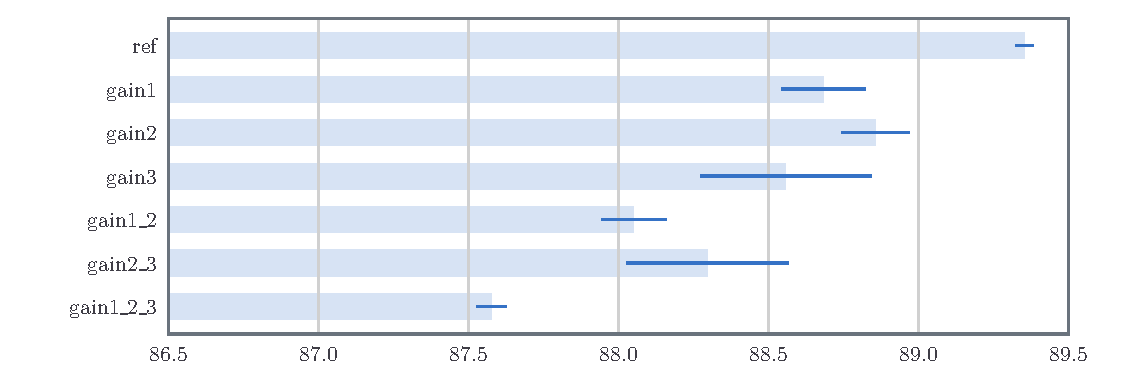
\includegraphics[width=\textwidth]{\imgpath/cifar10_gainlayer_large.pdf}
    \label{fig:ch6:cifar10_gl}
    }\\
  \subfloat[CIFAR-100]{%
    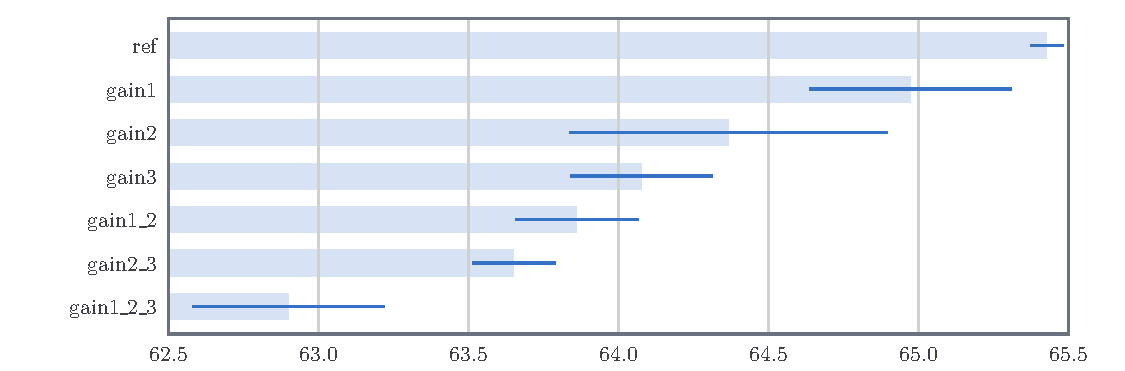
\includegraphics[width=\textwidth]{\imgpath/cifar100_gainlayer_large.pdf}
    \label{fig:ch6:cifar100_gl}
  }\\
  \subfloat[Tiny ImageNet]{%
    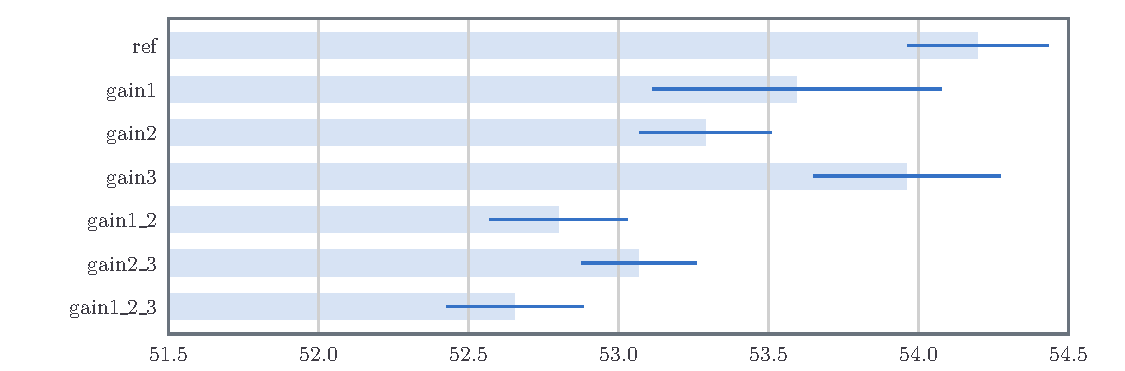
\includegraphics[width=\textwidth]{\imgpath/ti_gainlayer_large.pdf}
    \label{fig:ch6:ti_gl}
  }
  \mycaption{Large kernel ablation results CIFAR and Tiny ImageNet}{Results
  showing the percentage classification accuracies obtained by swapping
  combinations of the three conv layers in the reference architecture from
  \autoref{tab:ch6:ablation_arch} with gain layers. Results shown are averages
  of 3 runs with the $\pm1$ standard deviations shown as dark blue lines. These results
  show that changing a convolutional layer for a gain layer is possible, but
  comes with a small accuracy cost which compounds as more layers are swapped.}
  \label{fig:ch6:gl_results}
\end{figure}

\subsection{Network Analysis}
It is nonetheless interesting to see that a network with only gain layers
(`gain1\_2\_3') can achieve accuracies within a couple of percentage points of a
purely convolutional architecture.

In this section, we look at some of the properties of the `gain1\_2\_3' for
CIFAR-100 and compare them to the reference architecture.

\subsubsection{Bandpass Coefficients}
When analyzing the `gain1\_2\_3' architecture, the most noticeable thing is the
distribution of the bandpass gain magnitudes. \autoref{fig:ch6:bp_dists} shows
these for the second gain layer, gain2. Of the $64\x 128=8192$ complex
coefficients most have very small magnitude, in particular, the diagonal wavelet
gains. The disparity between the diagonal and horizontal/vertical wavelet gain
distributions echoes the observation made in
\autoref{sec:ch4:occlusion_results}, where we saw that occluding diagonal
subbands reduced classification performance by less than when occluding
horizontal/vertical subbands.

Although the diagonal subbands are particularly small, the horizontal and
veritcal bands have many coefficients with magnitude very close to zero.
This raises an interesting question -- how many of these coefficients are
important for classification? What if we were to apply a hard thresholding
scheme to the weights, would setting some of these values to zero impact the
network performance?

We measure the dropoff in accuracy when a hard threshold $t$ is applied to the
bandpass gains $g_1$ for the three gain layers of `gain1\_2\_3'. The resulting sparsity
of each layer and the network performance is shown in \autoref{fig:ch6:threshs}.
For example, if we set a hard threshold value $t=0.4$, only 20\% of the gain1
weights, 1\% of the gain2 and 0.02\% of the gain3 weights are non-zero, yet the
classification accuracy has only dropped by 0.5\%.

This figure shows that despite the high cost of the bandpass gains --
$12C_{l}C_{l+1}$ for a $1\x1$ gain, very few of these need to be nonzero.

\begin{figure}
  \centering
  \vspace{-0.5cm}
  \subfloat[Bandpass Magnitude Distributions]{
    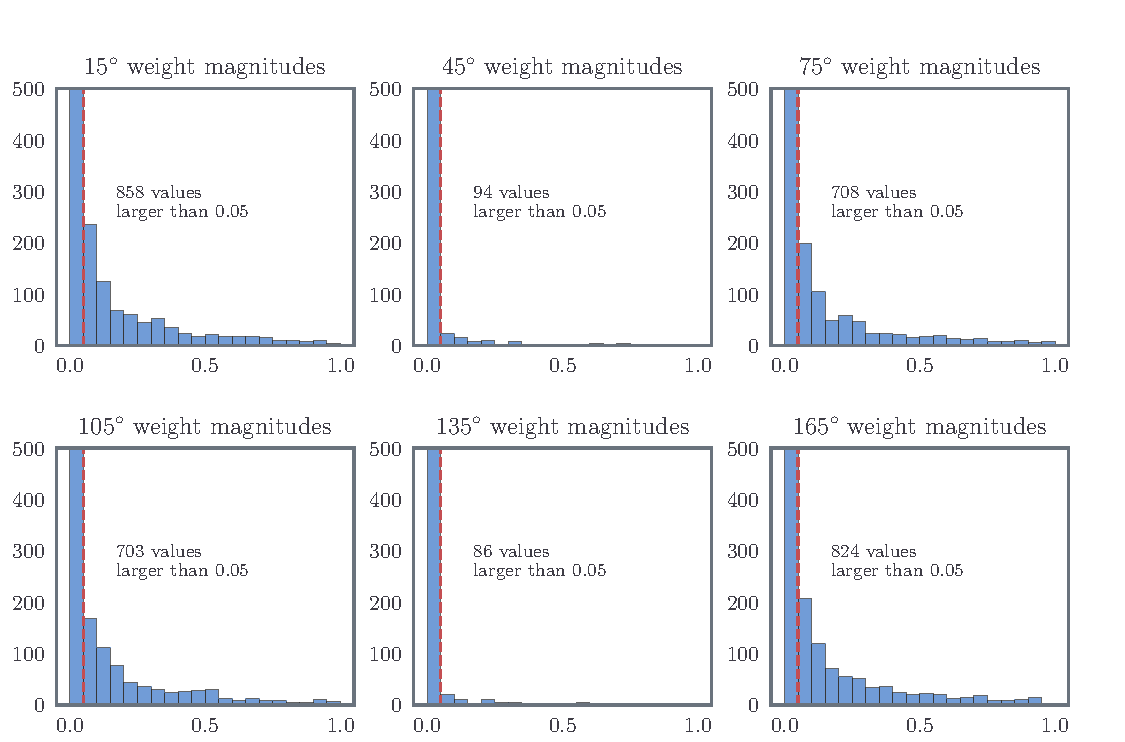
\includegraphics[width=.9\textwidth]{\imgpath/complex_mag_dists.pdf}
    \label{fig:ch6:bp_dists}
    }\\\vspace{-0.3cm}
  \subfloat[Accuracy Dropoff from Thresholding]{
    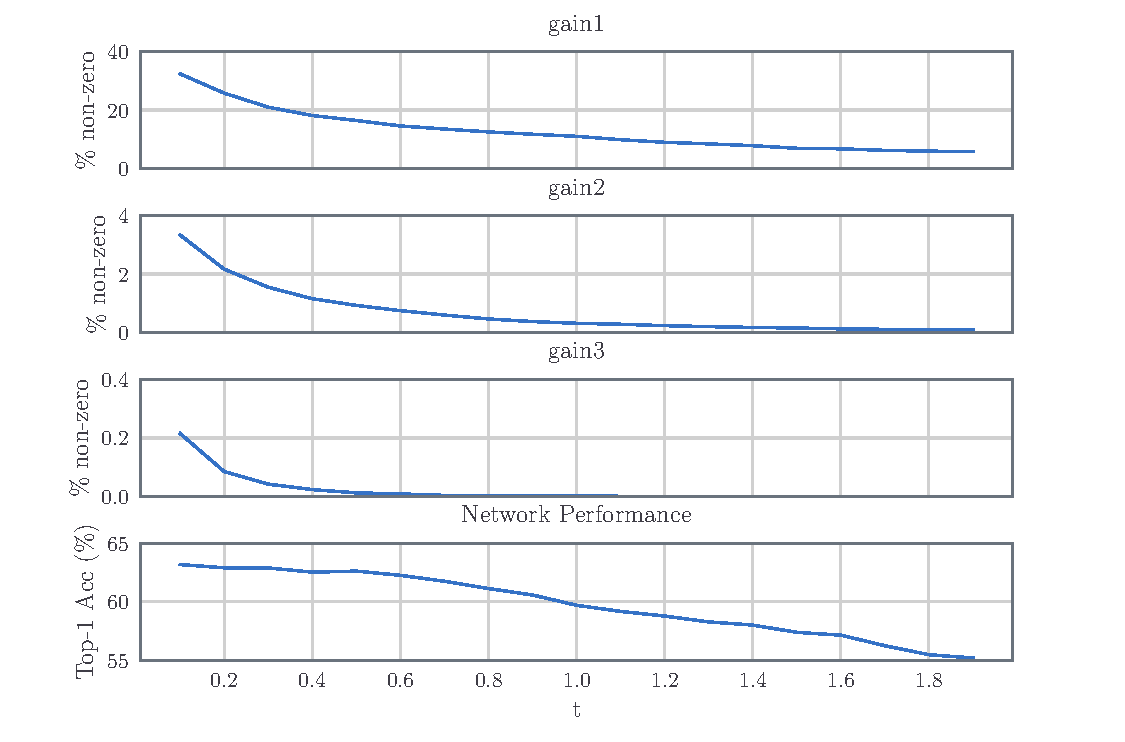
\includegraphics[width=\textwidth]{\imgpath/cifar100_gainlayer_threshs.pdf}
    \label{fig:ch6:threshs}
    }
    % \mycaption{}{}
    \mycaption{Bandpass Gain Properties for all gain layer network}{\subref{fig:ch6:bp_dists} shows the
    distribution of the magnitudes for bandpass coefficients for the second
    layer (gain2). Each orientation has $128\x 64=8192$ complex weights, most of
    which are close to 0 ($\ell_1$ regularization was used in training); Y axis
    for each plot has been clipped to 500. The $45\degs$ and $135\degs$ weights
    have many fewer large coefficients. \subref{fig:ch6:threshs} shows the
    increase in sparsity and dropoff in classification accuracy when the weights
    are hard-thresholded with value $t$ (same threshold applied to all 3
    layers).  For a threshold value of $t=0.4$, 80\% of the weights in gain1 are
    0, 99\% of the weights in gain2 are 0, 99.98\% of the weights in gain3 are
    0, yet classification accuracy is only 0.5\% lower than the non-thresholded
    accuracy.} \label{fig:ch6:bp_info}
\end{figure}

\subsubsection{DeConvolution and Filter Sensitivity}
To visualize what the gain layer is responsive to, we build a deconvolutional
system similar to the one described in \autoref{ch:visualizing}. In
particular, we present the entire CIFAR-100 validation set to the reference
architecture and to the gain1\_2\_3 architecture, keeping track of what most
highly excites each channel. Once we have this information, we present the same
image again, storing the ReLU switches and max pooling locations for this same
image, then we zero out all but a single value for the given channel, and zero out all
other channels, and deconvolve to see the input pattern.

The resulting visualizations for the first two layers are shown in
\autoref{fig:ch6:visualizations}. We show only the top activation for each
filter, rather than the top-9. For the second layer filters, we show only 64 of
the 128 filter responses.

It is reassuring to see that despite the
performance difference between the reference architecture and the gain1\_2\_3
architecture, the filters are responding to similar shapes. Note that for both the
first and second layer responses, the gain layer has a smoother roll-off at the
edges of the visualization, whereas the convolutional architecture has more
square regions of support.

\begin{figure}
  \centering
  \subfloat[First layer]{
  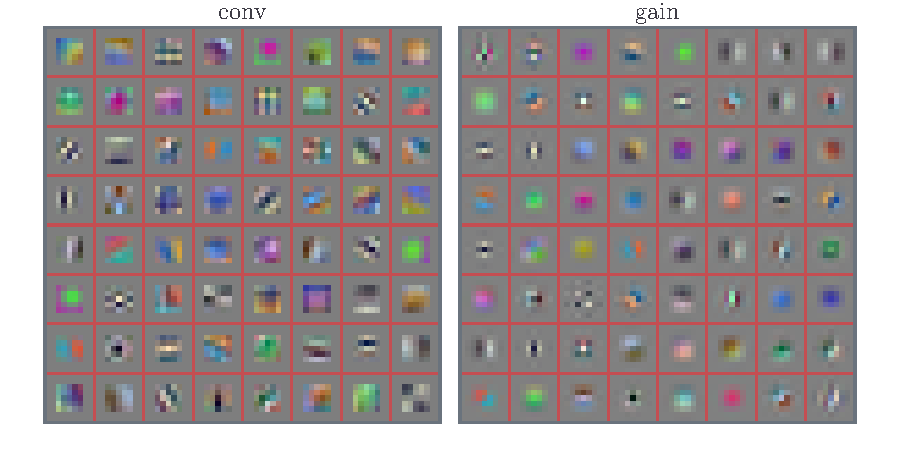
\includegraphics{\imgpath/largekernel_conv1.pdf}
  } \\
  \subfloat[Second layer]{
  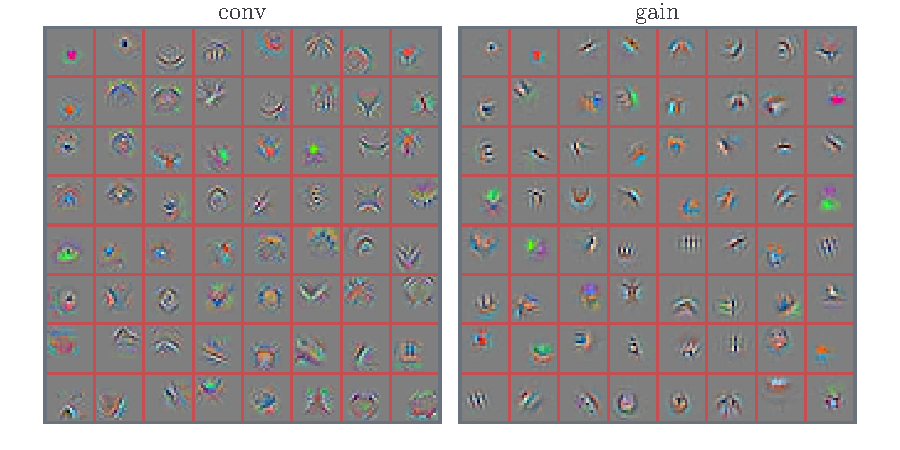
\includegraphics{\imgpath/largekernel_conv2.pdf}
  }
  \mycaption{Deconvolution reconstructions for the reference architecture and
  purely gain layer architecture}{Visualizations using a DeConvNet method similar to
  the one described in \autoref{ch:visualizing}. Here we find the input images in CIFAR-100 validation
  set that most highly activate each filter. Each image is then re-shown to the
  network and the meta-information is used to prime the DeConvNet to create the visualizations seen here.
  The left column has visualizations for the first and second layer filters for
  the all convolutional method, and the right column has visualizations for
  the first and second layer filters for the all gain layer method. Note the
  smoother roll-off at the edge of visualizations in the gain layer compared to
  the rectangular support regions for the conv layers. Aside from that, the two
  networks appear to be learning similar shapes.}
  \label{fig:ch6:visualizations}
\end{figure}


